\newpage
\problem{2: Remote Sensors} % {10+10+10+20=50}

\problemdes

\begin{figure}[!ht]
    \centering
    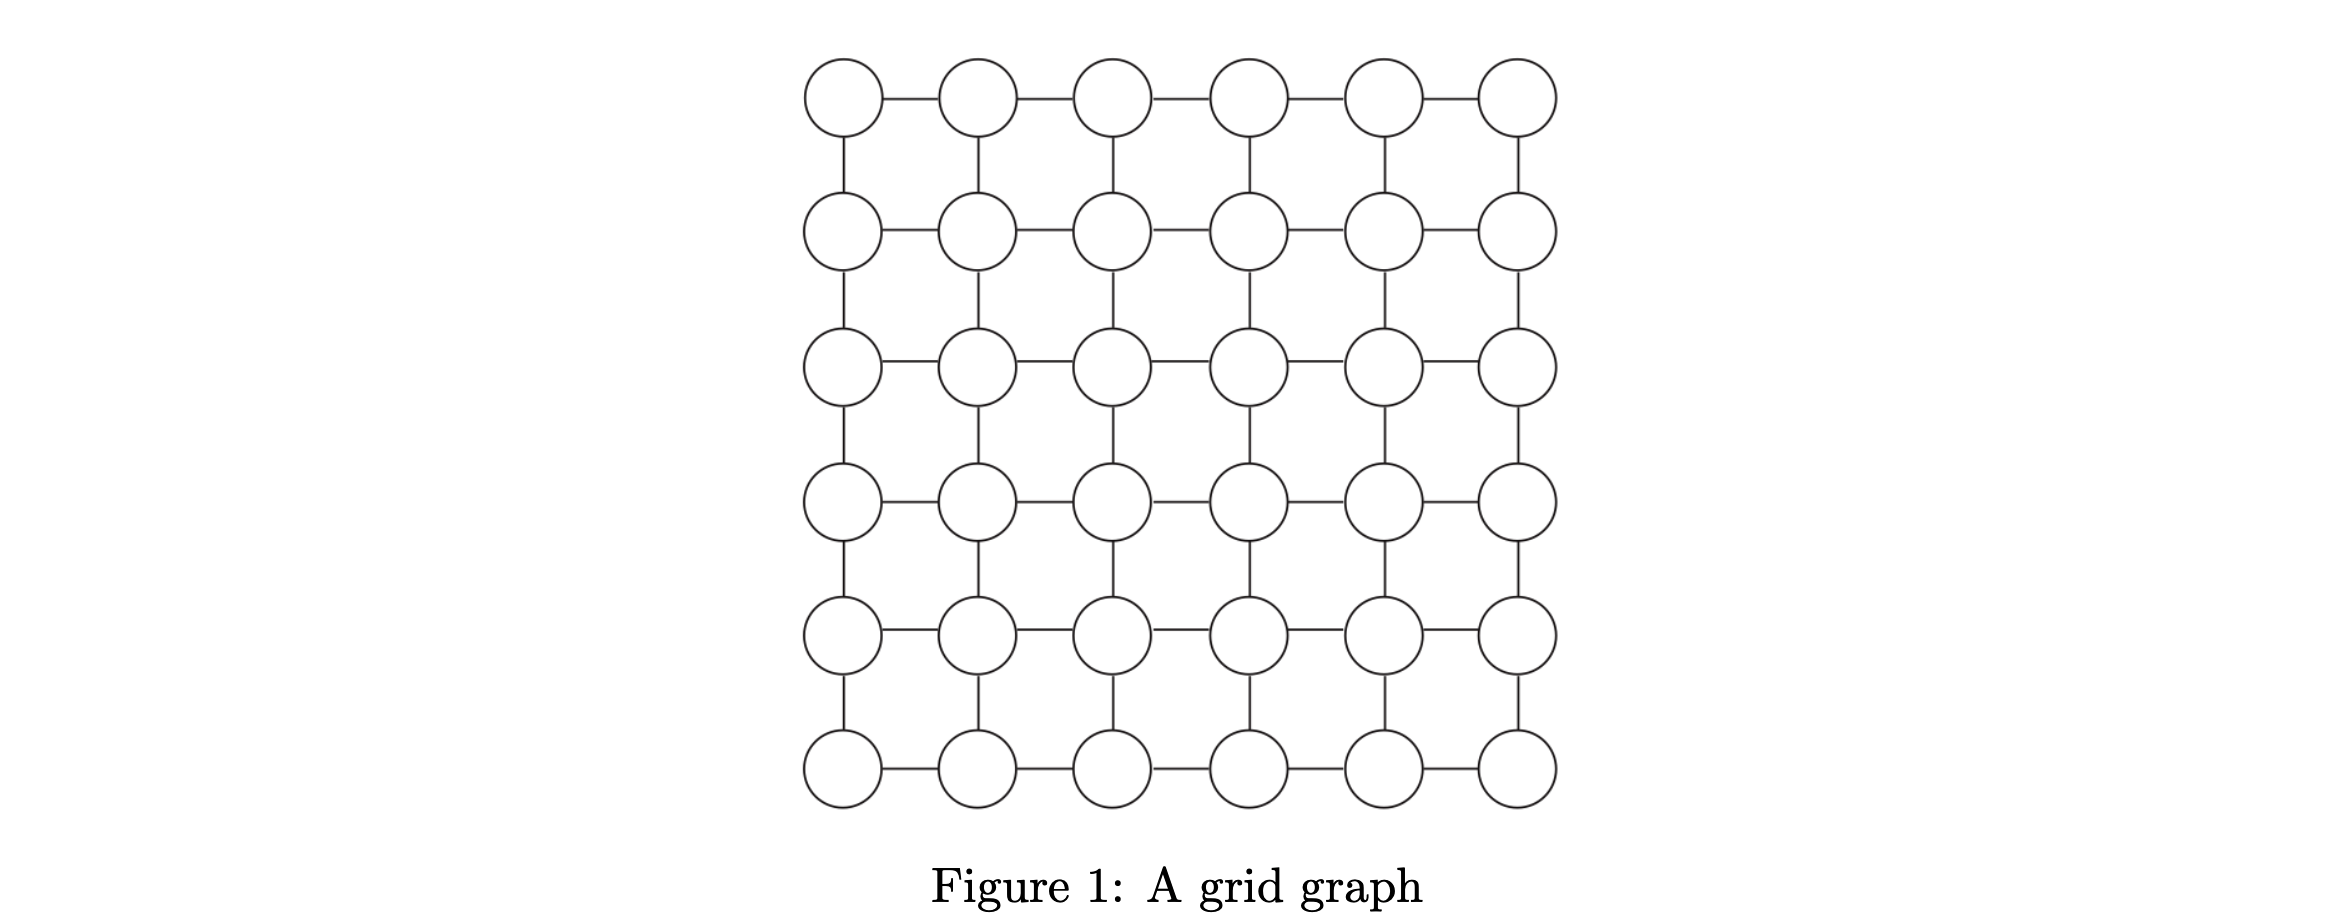
\includegraphics[width=\textwidth]{graph.png}
    \label{fig:algo}
\end{figure}

Suppose you are given an $n \times n$ grid graph $G$, as in Figure 1 Associated with each node $v$ is a weight $w(v)$, which is a nonnegative integer. You may assume that the weights of all nodes are distinct. Your goal is to choose an independent set $S$ of nodes of the grid, so that the sum of the weights of the nodes in $S$ is as large as possible. (The sum of the weights of the nodes in $S$ will be called its total weight.) Consider the following greedy algorithm for this problem.

\begin{figure}[!ht]
    \centering
    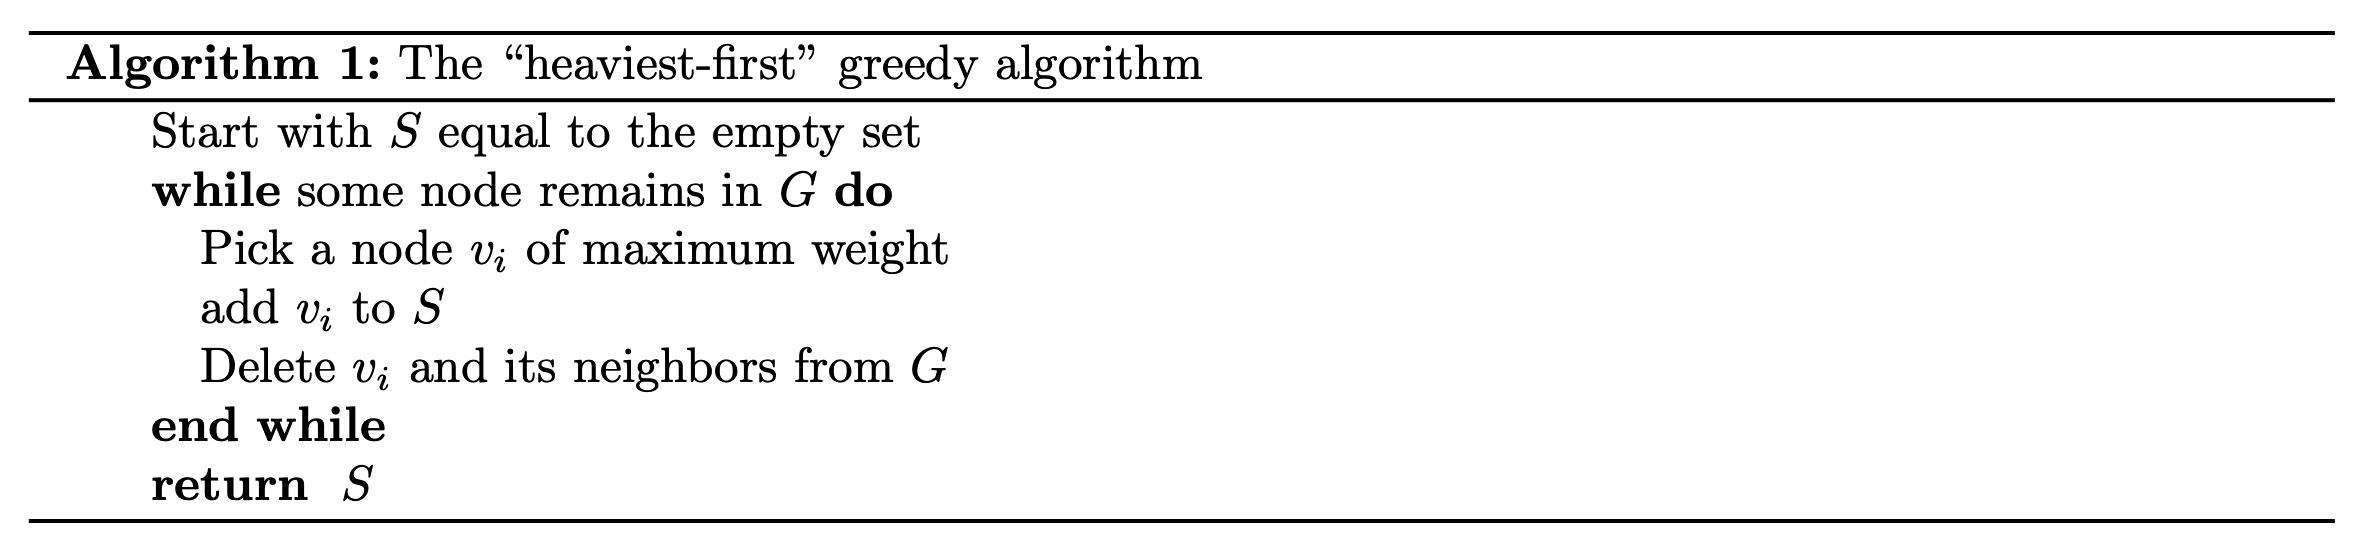
\includegraphics[width=\textwidth]{algorithm.png}
    \label{fig:algo}
\end{figure}

\subproblem{Subproblem 1}

Let $S$ be the independent set returned by the “heaviest-first” greedy algorithm, and let $T$ be any other independent set in $G$. Show that, for each node $v \in T$, either $v \in S$,or there is a node $v^\prime \in S$ so that $w(v) \le w(v^\prime)$ and $(v, v^\prime)$ is an edge of $G$.

\subsolution{Solution 1}

%\subsolution{High-level description}

%\subsolution{Pseudo Code}

% \subsolution{Correctness}


% \subsolution{Time complexity}

\textit{Proof.} For node $v\in T$, if $v \notin S$, then it means that it is deleted at some iteration when selecting its neighbor $v^\prime$. And following the instruction of greedy algorithm, $v^\prime$ must contain a larger weight than $v$. Otherwise we will choose to add $v$ to $S$. Hence, we proved that for each node $v\in T$, either $v\in S$ or there is a node $v^\prime \in S$ so that $w(v) \le w(v^\prime)$ and $(v, v^\prime)$ is an edge of $G$.

\subproblem{Subproblem 2}

Show that the “heaviest-first” greedy algorithm returns an independent set of total weight at least $1/4$ times the maximum total weight of any independent set in the grid graph $G$.

\subsolution{Solution 2}

%\subsolution{High-level description}

%\subsolution{Pseudo Code}

%\subsolution{Correctness}

%\subsolution{Time complexity}

We use $T$ to denote any independent set in the grid graph $G$, let $S$ denote the independent set found by the heaviest-first greedy algorithm. We want to show that $W_S \ge \forall_{T} \frac{1}{4} W_{T}$.

% We need to notice that both $T$ and $S$ are independent set, which means for each node $v \in T$, its neighbors $v^\prime \notin T$. 

For any node $v \in T$, 

\textit{Case 1}. If $v\in S$, since $G$ is a grid graph, then at most four neighboring nodes of no greater weights $v^\prime_{1, 2, 3, 4} \in T$.

\textit{Case 2}. If $v\notin S$, as proved in subproblem 1, there must be a node $v^\prime \in S$ so that $w(v) \le w(v^\prime)$ and $(v, v^\prime)$ is an edge of $G$. For $v^\prime$, there are at most four neighboring nodes of no greater weights $\in T$.

Either case, the total weight of all nodes in $T$ should not be greater than four times than the total weights of all nodes in $S$. Hence, we proved that $W_S \ge \forall_{T} \frac{1}{4} W_{T}$.










